\documentclass[12pt]{article}
%%%%%%%%%%%%%%%%%%%%%%%%%%%%%%%%%%%%%%%%%%%%%%%%%%%%%%%%%%%%%%%%%%%%%%%%%%%%%%%%%%%%%%%%%%%%%%%%%%%%%%%%%%%%%%%%%%%%%%%%%%%%%%%%%%%%%%%%%%%%%%%%%%%%%%%%%%%%%%%%%%%%%%%%%%%%%%%%%%%%%%%%%%%%%%%%%%%%%%%%%%%%%%%%%%%%%%%%%%%%%%%%%%%%%%%%%%%%%%%%%%%%%%%%%%%%
\usepackage{tikz}
\usepackage{algorithm,algpseudocode} % Did not work inside tikzpicture 
\usepackage{setspace}
\usepackage{xcolor}
\usepackage{amssymb}
\usepackage{amsmath}
\usepackage{amsfonts}
\usepackage{titlesec}
\usepackage[margin=1.5in]{geometry}
\usepackage{graphicx}
\usepackage[hidelinks]{hyperref}
\usepackage{etoolbox}
\usepackage{xr}
\usepackage{natbib}
\usepackage{lmodern}
\usepackage{standalone}
\usepackage{multirow}
\usepackage{graphicx}
\usepackage{caption,subcaption}
\usepackage{booktabs}
\usepackage{pdflscape}
\setcounter{MaxMatrixCols}{10}
\begin{document}

%\begin{itemize}
%  \item Figure
%\end{itemize}

    \begin{table}
      \caption{Recall rates for E-U-E spells}
      \begin{center}
\begin{tabular}{l|cc}
  \hline \hline
   & \multicolumn{2}{c}{\textit{From}:} \\[0.35em]
                                     &\multicolumn{1}{c}{Temporary} & \multicolumn{1}{c}{Permanent} \\
   \textit{Panel:}                                  
                                     &\multicolumn{1}{c}{layoff} & 
                                     \multicolumn{1}{c}{separation} 
                                     \\[0.35em]
                                     \hline \\[-1em]
  All  & 0.763 & 0.064 \\[.35em]
  1996 & 0.740 & 0.063 \\[.35em]
  2001 & 0.754 & 0.068 \\[.35em]
  2004 & 0.766 & 0.080 \\[.35em]
  2008 & 0.782 & 0.047 \\[.35em]
               \hline
\end{tabular}
    \subcaption*{\small \textit{Note:} [Subcaption TBW]}
      \end{center}
    \end{table}

    \begin{table}
      \caption{Cyclical Properties of Recall}
      \begin{center}
    \begin{tabular}{l|rrrrrr}
      \hline
      \hline \\ [-1em] 
      & \multicolumn{1}{c}{$u$} & \multicolumn{1}{c}{$p_{\text{recall}}$} & \multicolumn{1}{c}{$p_{TL,E}$} & \multicolumn{1}{c}{$p_{JL,E}$} & \multicolumn{1}{c}{$p_{E,TL}$} & \multicolumn{1}{c}{$p_{E,JL}$} \\[0.35em]  
      \hline \\[-1em]
      Sample mean                 & $6.11$ & $0.421 $ & $0.491 $ & $0.322$ & $0.003$ & $0.005$ \\[.35em]
      Correlation with $u$ & $1.00$ & $-0.253$ & $-0.271$ & $0.484$ & $0.346$ & $0.341$ \\[.35em]
      \hline
      \hline
    \end{tabular}
      \end{center}
  \end{table}

  \begin{figure}
    \caption{U-to-E Hazards: Recall and New Job-Finding\label{fig:UE}}
  \centerline{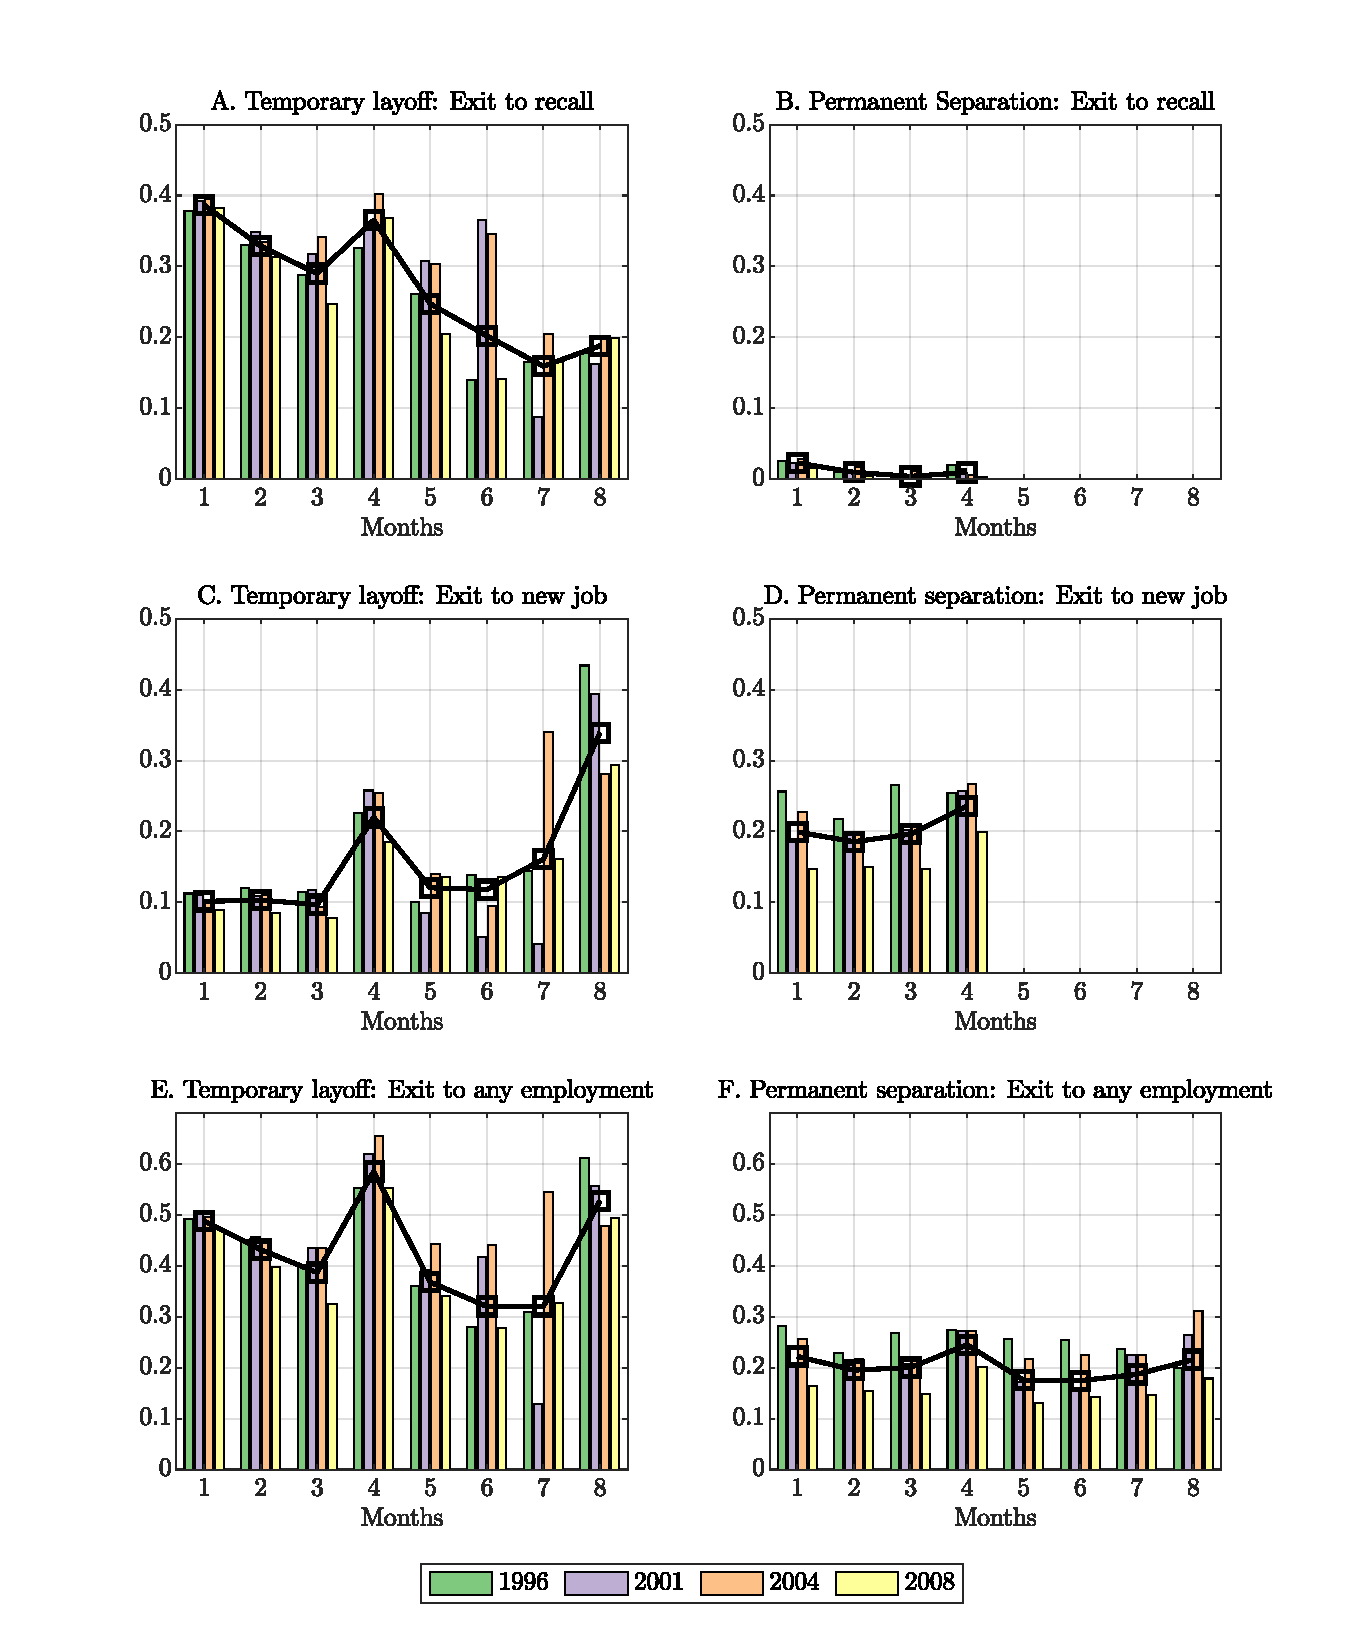
\includegraphics[width=1.00\linewidth]{./../figures/all}}
    \subcaption*{\small \textit{Note:} [Subcaption TBW]}
  \end{figure}

  \begin{figure}
  \caption{SIPP interview structure}
    \begin{center}
      \includegraphics[width=\linewidth]{sipp_waves}

% \begin{tikzpicture}
%     \def\length{13}
%     \def\pattern{1,...,13}
% 
%     % Draw the horizontal line
%     \draw[-] (0.5,0) -- (\length+0.5,0);
%         
%     
%     % Draw labels, ticks and text
%     \foreach \x in \pattern {
%         \pgfmathtruncatemacro{\modvalue}{mod(\x, 4)}
%         % Draw the repeating labels
%         \ifnum\modvalue=0
%             \node at (\x, 0.1) -- (\x,-0.1) node[below] {4};
%         \else
%             \node at (\x, 0.1) -- (\x,-0.1) node[below] {\modvalue};
%         \fi
% 
%         % Draw the major and the minor ticks
%         \ifnum\ifnum\x=1 1 \else\ifnum\x=5 1 \else\ifnum\x=9 1 \else\ifnum\x=13 1 \else 0\fi\fi\fi=1
%             \draw (\x-0.5,-0.25) -- (\x-0.5,0.25);
% %        \else
% %            \ifnum\x=\length
% %                \draw (\x-0.5,-0.1) -- (\x-0.5,0.1);
% %                \draw (\x+0.5,-0.1) -- (\x+0.5,0.1);
% %            \else
%                 \draw (\x-0.5,-0.1) -- (\x-0.5,0.1);
% %            \fi
%         \fi
% 
%         % Draw the text labels
%         \ifnum\x=2
%             \node[above] at (2.5,0.4) {Wave $t-1$}
%         \fi
%         
%         \ifnum\x=6
%             \node[above] at (6.5,0.4) {Wave $t$}
%         \fi
%         
%         \ifnum\x=11
%             \node[above] at (10.5,0.4) {Wave $t+1$}
%         \fi
%     }
% \end{tikzpicture}
    \end{center}
  \end{figure}

    \begin{table}
      \caption{First reference month of unemployment spell}
      \begin{center}
  \begin{tabular}{l|cccc}
    & \multicolumn{1}{c}{1$^\text{st}$ ref.}
    & \multicolumn{1}{c}{2$^\text{nd}$ ref.}
    & \multicolumn{1}{c}{3$^\text{rd}$ ref.}
    & \multicolumn{1}{c}{4$^\text{th}$ ref.} \\
    & \multicolumn{1}{c}{month}
    & \multicolumn{1}{c}{month}
    & \multicolumn{1}{c}{month}
    & \multicolumn{1}{c}{month} \\ \hline \\[-1em]
    Permanent separations & 0.387 &  0.205 &  
    0.202 &   0.207 \\[.35em]
    Temporary layoffs     & 0.328 &  0.210 &  0.233 &   0.230 \\[.35em]
    \hline
  \end{tabular}
    \subcaption*{\small \textit{Note:} [Subcaption TBW]}
      \end{center}
    \end{table}

    \begin{table}
      \caption{Final reference month of unemployment spell}
      \begin{center}
  \begin{tabular}{l|cccc}
    & \multicolumn{1}{c}{1$^\text{st}$ ref.}
    & \multicolumn{1}{c}{2$^\text{nd}$ ref.}
    & \multicolumn{1}{c}{3$^\text{rd}$ ref.}
    & \multicolumn{1}{c}{4$^\text{th}$ ref.} \\
    & \multicolumn{1}{c}{month}
    & \multicolumn{1}{c}{month}
    & \multicolumn{1}{c}{month}
    & \multicolumn{1}{c}{month} \\ \hline \\[-1em]
    Permanent separations & 0.203 &  0.209 &  
    0.223 &   0.365 \\[.35em]
    Temporary layoffs     & 0.137 &  0.190 &  
    0.236 &   0.437 \\[.35em]
    \hline
  \end{tabular}
    \subcaption*{\small \textit{Note:} [Subcaption TBW]}
      \end{center}
    \end{table}


  \begin{landscape}
    \begin{figure}
    \caption{U-to-E Hazards by Reference Month at Start of Spell: 
    Temporary Layoffs\label{fig:UEtl}}
    \centerline{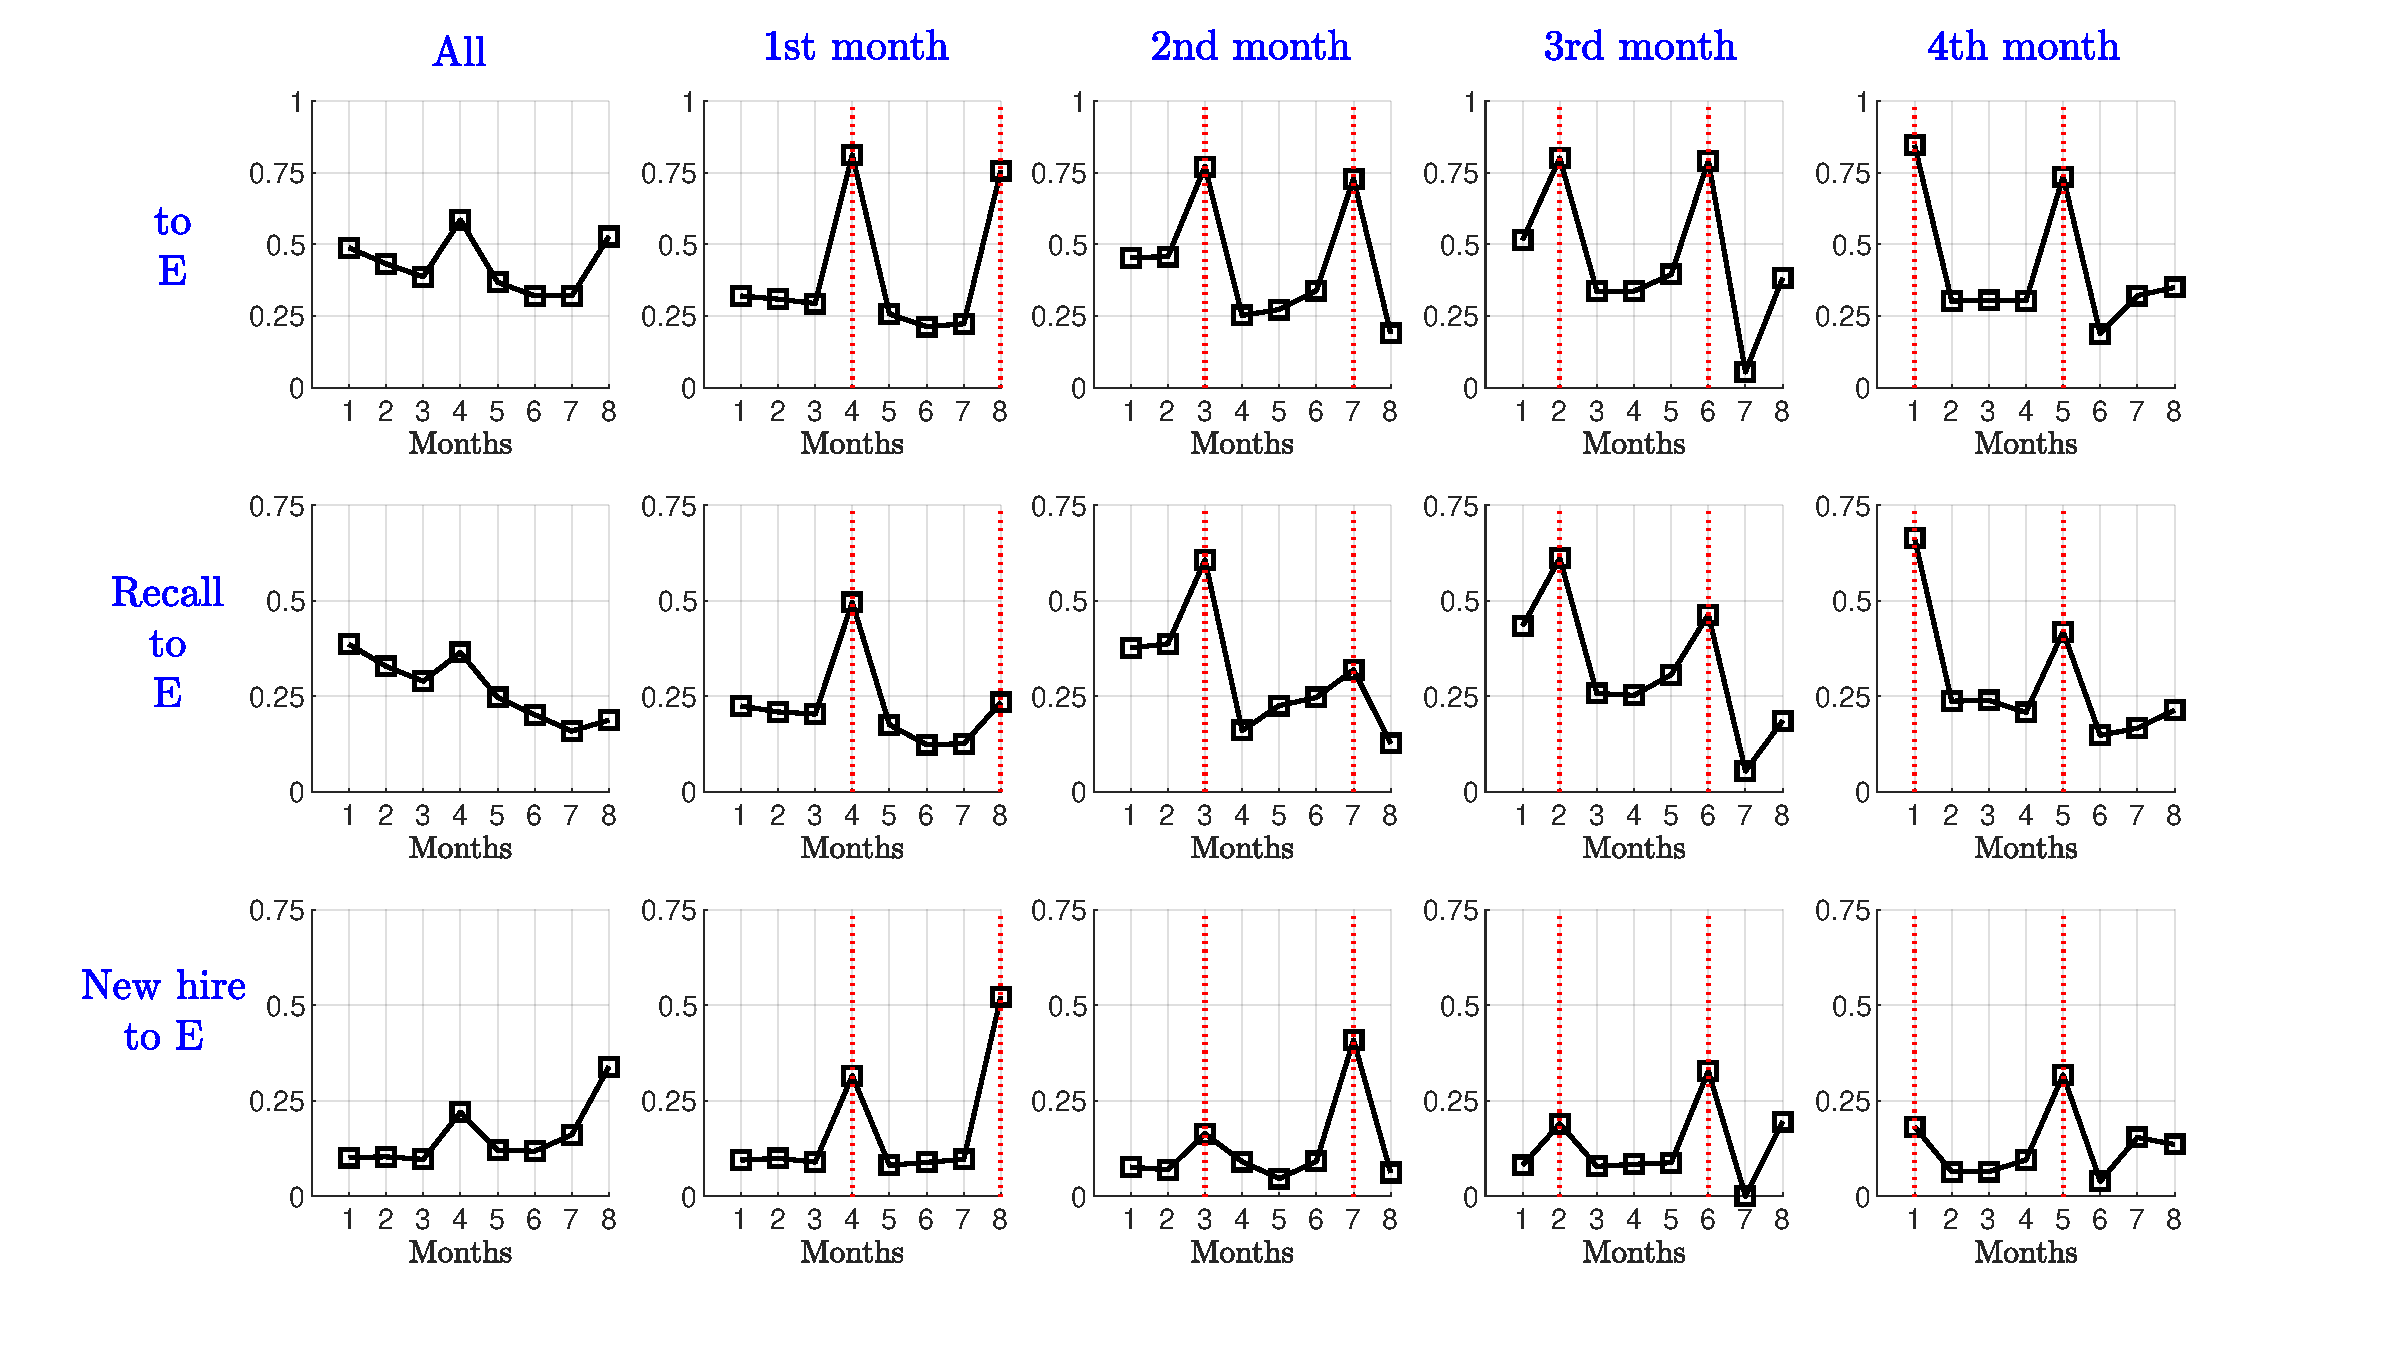
\includegraphics[width=1.00\linewidth]{./../figures/TL}}
    \subcaption*{\small \textit{Note:} [Subcaption TBW]}
    \end{figure}

  \begin{figure}
  \caption{U-to-E Hazards by Reference Month at Start of Spell: 
  Permanent Separations\label{fig:UEtl}}
  \centerline{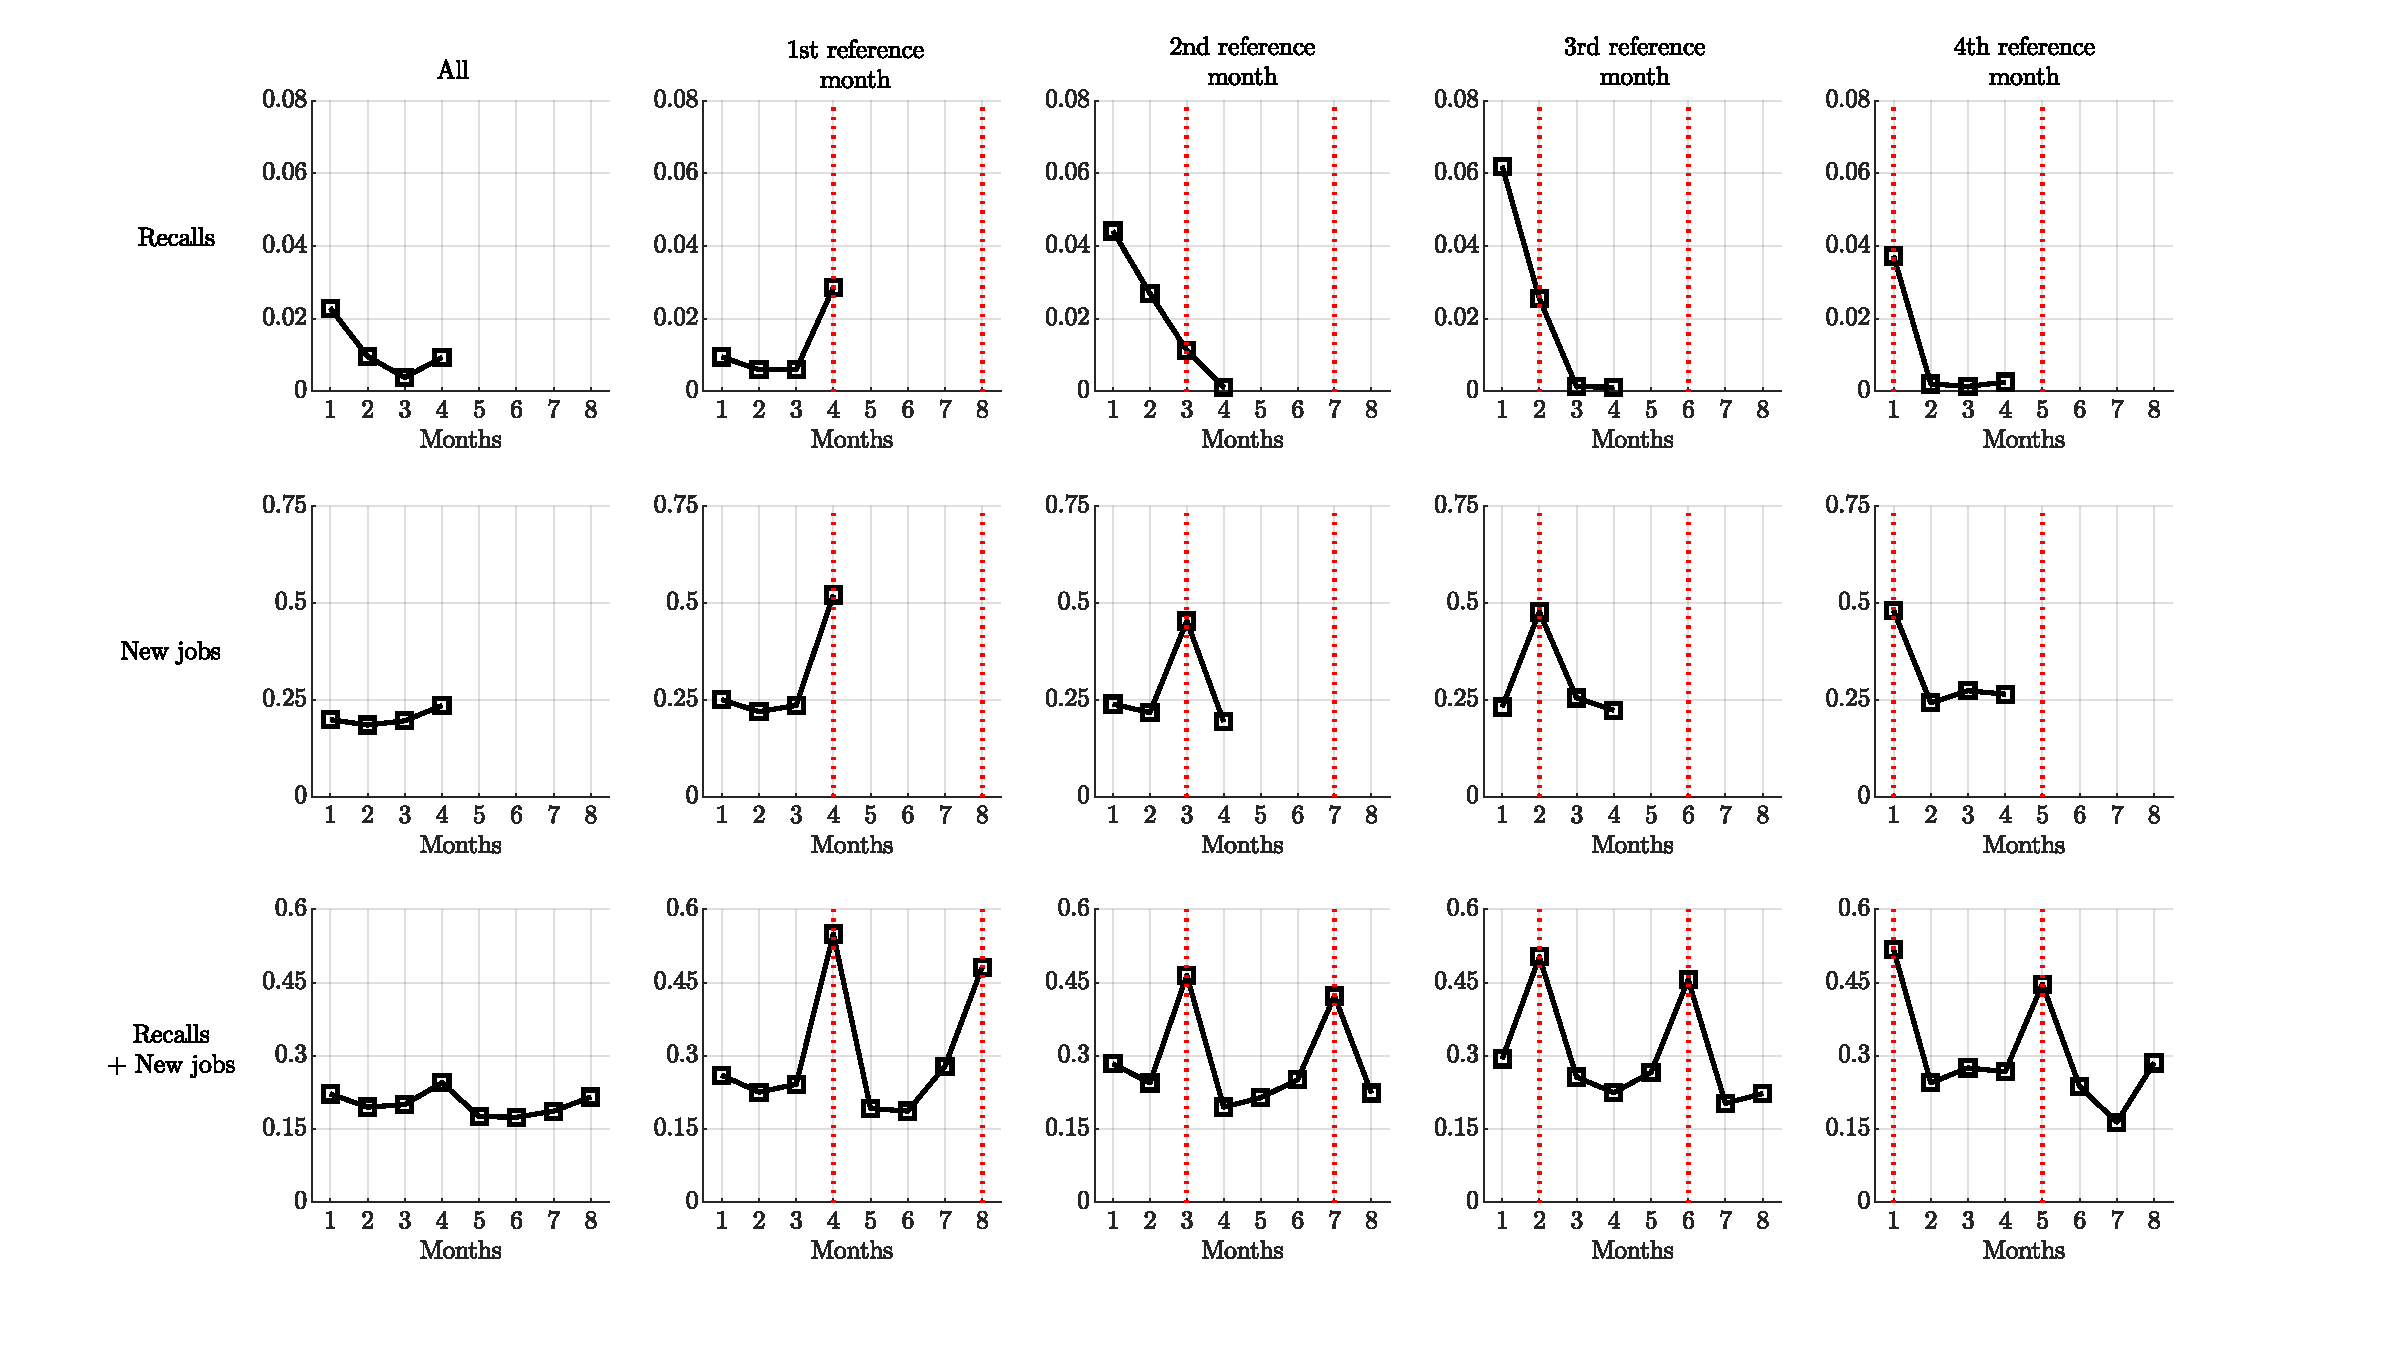
\includegraphics[width=1.00\linewidth]{./../figures/PS}}
    \subcaption*{\small \textit{Note:} [Subcaption TBW]}
  \end{figure}
  \end{landscape}

\end{document}
